% Graphic Processing Unit
%
%	Take from the PA

\chapter{Graphics Processing Unit}

A \gls{GPU} is a specialized chip for outputting an image on a display. They are used in embedded systems, mobile phones, personal computers, workstations, and game consoles. \Glspl{GPU} are presently able to compute 3D images using a custom programmable rendering pipeline. This capacity can be diverted to be used for general purpose computing.

\section{Introduction}

General purpose programming on \glspl{GPU} is a new field with a growing community of practitioners. Until recently only proprietary interfaces existed to harness the power of these chips. With the arrival of the \gls{OpenCL} a new open interface has appeared, and with it a hope for a unified, simple and portable framework for general purpose computing on heterogeneous hardware.

\section{OpenCL}

The \gls{OpenCL} is the open standard for \gls{GPGPU} programming. It is maintained by the Khronos group, and was initially proposed by Apple. Many companies of the industry are members of the \gls{OpenCL} Working group: Altera, AMD, Apple, ARM, Broadcom, Codeplay, DMP, EA, Ericsson, Fixstars, Freescale, Hi corp, IBM, Intel, Imagination Technologies, Kestrel Institute, Kishonti, Los Alamos National Laboratory, Motorola, Movidius, Multicoreware, Nokia, NVIDIA, OpenEye, Presagis, Qualcomm, Rightware, Samsung, ST, Symbio, Texas Instruments, The University of West Australia, Vivante and Xilinx.\cite{opencl}
\begin{quotation}
``OpenCL\texttrademark is the first open, royalty-free standard for cross-platform, parallel programming of modern processors found in personal computers, servers and hand-held / embedded devices. \gls{OpenCL} greatly improves speed and responsiveness for a wide spectrum of applications in numerous market categories from gaming and entertainment to scientific and medical software.''\cite{opencl}
\end{quotation}
\begin{quotation}
``The Khronos Group is a not for profit industry consortium creating open standards for the authoring and acceleration of parallel computing, graphics, dynamic media, computer vision and sensor processing on a wide variety of platforms and devices. All Khronos members are able to contribute to the development of Khronos \gls{API} specifications, are empowered to vote at various stages before public deployment, and are able to accelerate the delivery of their cutting-edge 3D platforms and applications through early access to specification drafts and conformance tests.''\cite{khronos}
\end{quotation}

\subsection{Architecture}

\gls{OpenCL} is not really a language but an \gls{API} and a kernel language derived from C99 that is compiled for, and executed on the device itself. It defines an abstract hardware architecture onto which the real hardware is mapped. Every piece of hardware (\gls{CPU}, \gls{GPU}, others) is called a device. This device is divided into work groups, each of which is further subdivided into work items.

\begin{figure}[H]
\caption{OpenCL Device Model}
\floatfoot{Source : OpenCL in Action\cite{OpenCLInAction}}
\centering
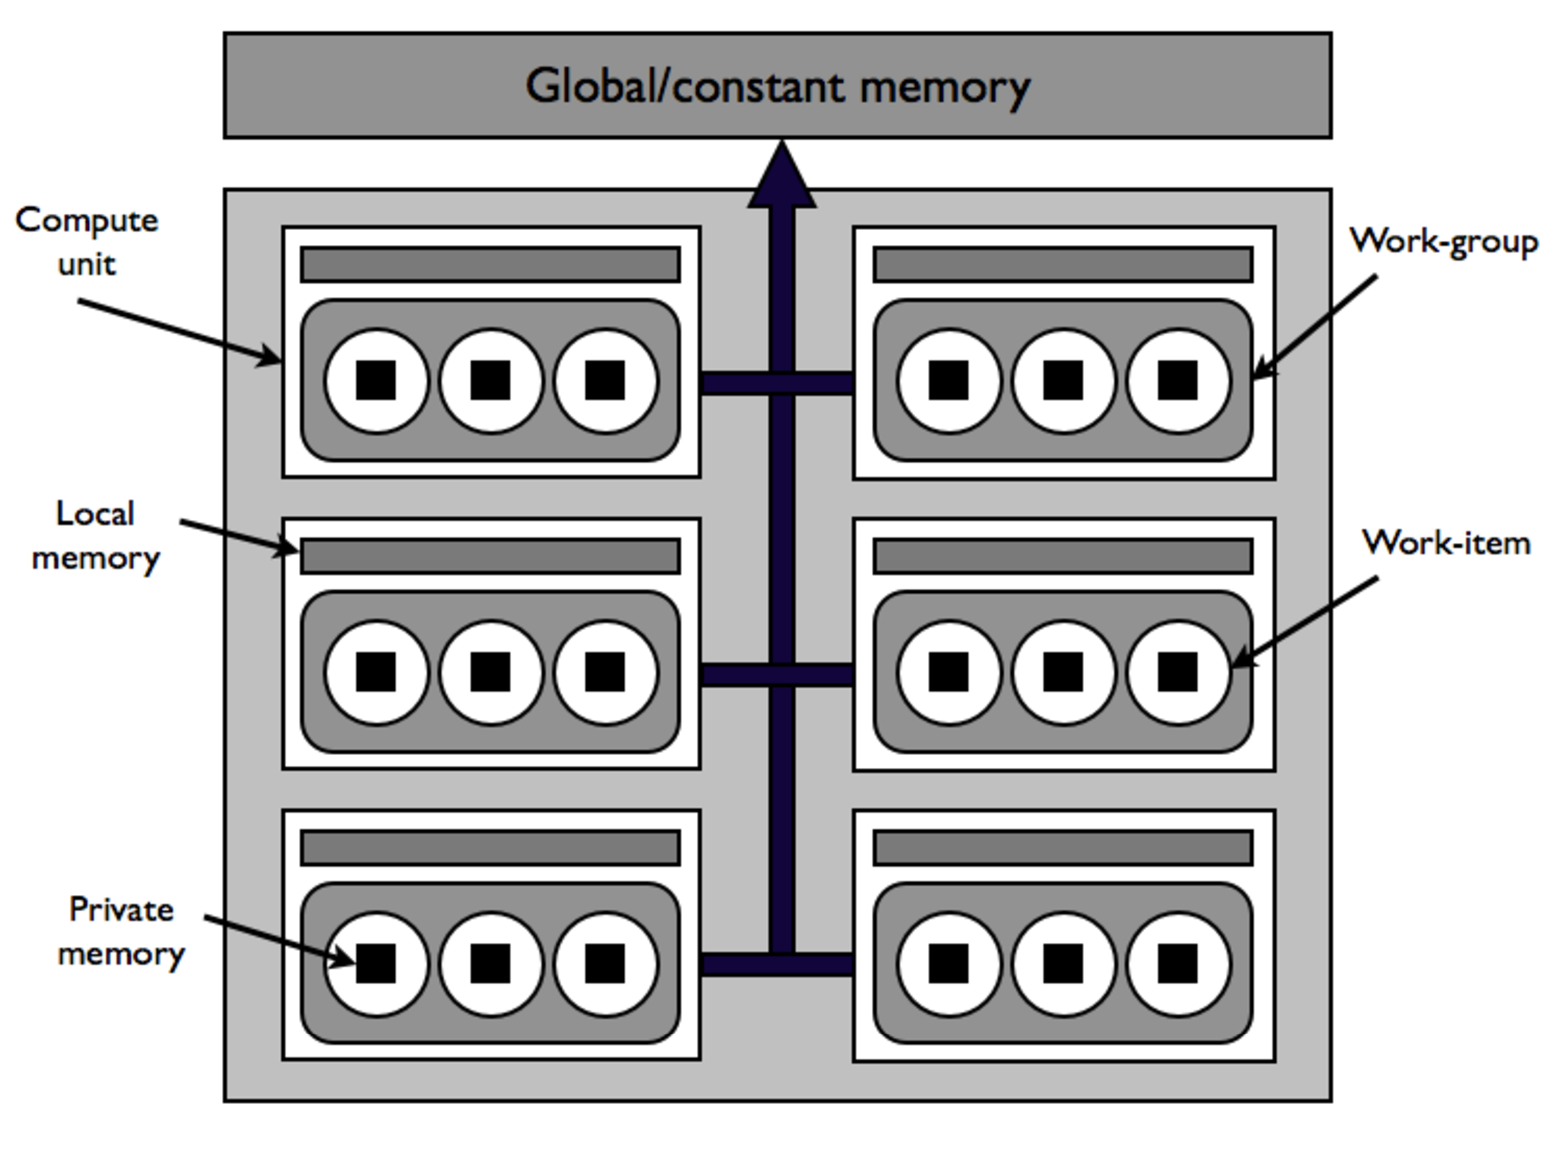
\includegraphics[scale=0.5]{OpenCL_Device_Model.pdf}
\end{figure}

\subsection{OpenCL API}

The \gls{OpenCL} \gls{API} is composed of two parts: The host code that runs on the CPU which runs kernel handling event synchronization and manages the memory buffer, and the device code, which is a kernel language based on the C99 specification.

\begin{figure}[H]
\caption{Kernel Distribution among OpenCL-compliant devices}
\floatfoot{Source : OpenCL in Action\cite{OpenCLInAction}}
\centering
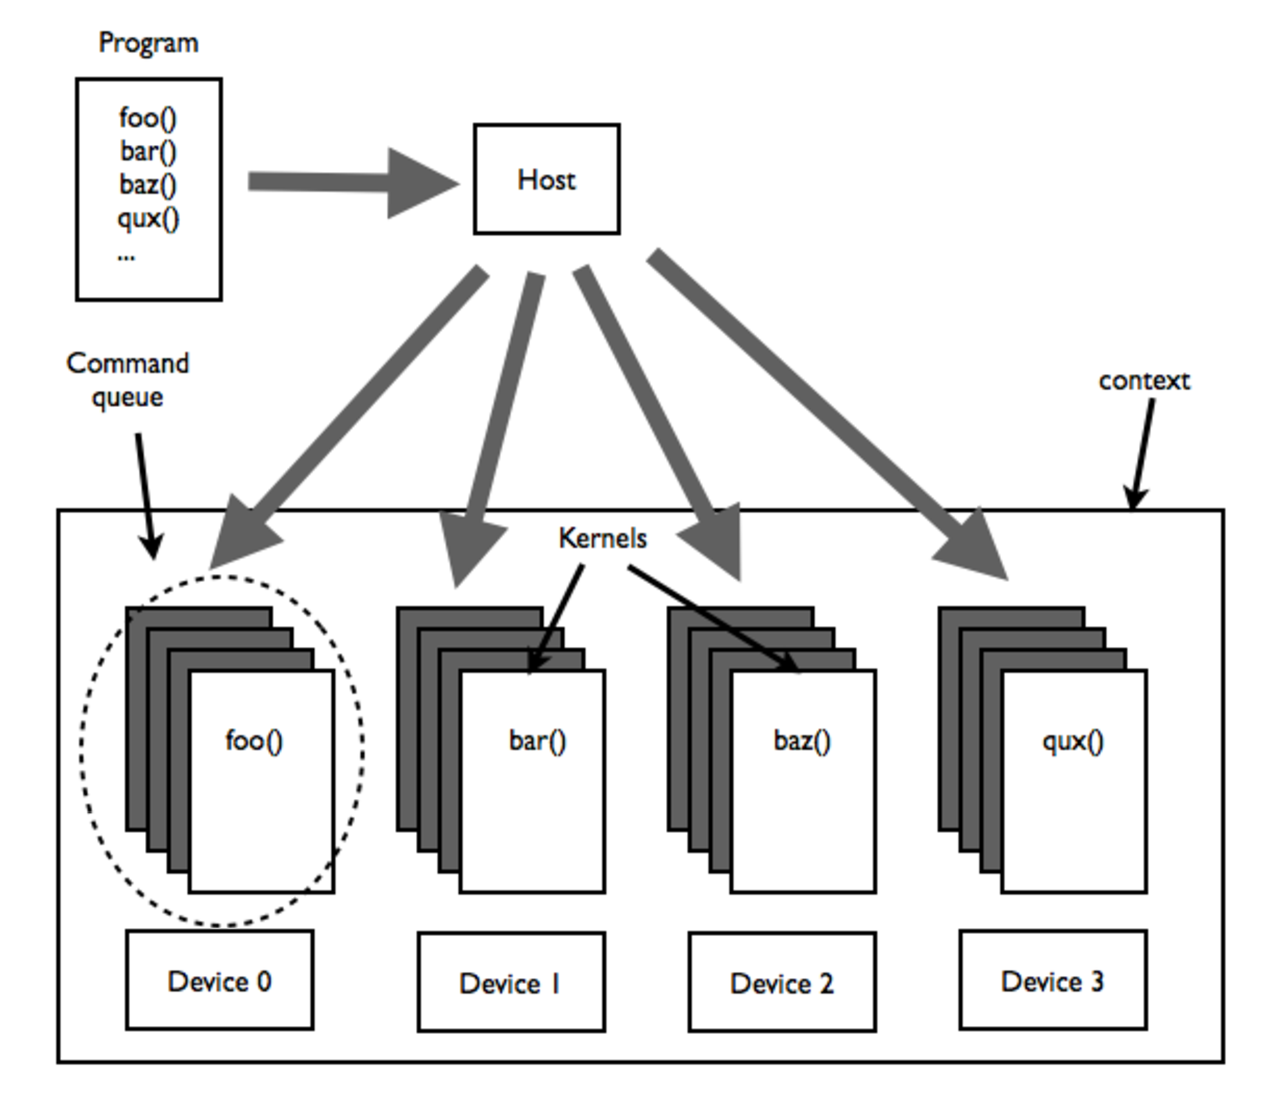
\includegraphics[scale=0.5]{OpenCL_Objects.pdf}
\end{figure}

The host \gls{API} is written in C but there is a C++ interface provided by Khronos, which is the interface used in this work. Several other wrappers for other languages are available, such as Java, C\#, Python, and even javascript with WebCL (also specified by the Khronos group). 

The device code also called \gls{OpenCL} ``kernel code'' is based on is C99, adding some extensions like vectorization, image access, and linear algebra functions.

The workload itself is specified in terms of context, program and command queues. The context contains the parameters of the current problem and manages the devices available for computation, as well as the programs and the command queues. The program consists of the set of kernels which are constructed from \gls{OpenCL} code. The context is responsible for dispatching these kernels into command queues. Each command queue is a set of commands that can be executed in any order, or simultaneously. A command queue is limited to a single device.\cite{OpenCLInAction,OpenCLProgrammingGuide}

Events fired by devices are also available for triggering specific actions in case a finer synchronization mechanism is needed. Once the device has finished, the host receives and processes the output data via the buffer \gls{API}.

\section{Other GPGPU languages}

For the purpose of completeness we present also the other general purpose computing languages used on \glspl{GPU}. Shader languages, the 3D pipeline programming languages used for computer graphic, will also be briefly mentioned. hey are not a real general purpose computing language but are still used for general purpose computing.

\subsection{CUDA}

\Gls{CUDA} is the most widely used interface for general purpose \gls{GPU} programming. It was developed by NVIDIA, has been used for many years and is still very much in use. It only works on NVIDIA \glspl{GPU}, and will not run on other \glspl{GPU} or \glspl{CPU}. Since it is a proprietary language, NVIDIA is in total control of the API and its development kit.

The abstraction level in \gls{CUDA} is less strong than in \gls{OpenCL}, that is, the language is closer to the architecture. This means it could potentially offer more optimization possibilities to the programmer. We will see that this is not a key element as the compiler is able to reach this level of optimization without having to compromise code readability.

\Gls{CUDA} has its kernel and \gls{GPU} code directly embedded inside the C/C++ code. In \gls{OpenCL} the code is separated from the C/C++ host code. This can lead to incompatibilities with C++ as valid C++ code will be flagged as invalid by the \gls{CUDA} compiler. This problem does not exist for \gls{OpenCL} as the compiler is a separate entity and the code is fed to it via the \gls{API}. 

\Gls{CUDA} offers a full suite of libraries and tools that are presently not available in \gls{OpenCL}. Among these are performance tuning tools and libraries for matrices and \glspl{FFT}. Recently many implementations of common algorithms have started to appear for \gls{OpenCL}, and unlike with \gls{CUDA}, these are directly available to any computing device.

\subsection{DirectCompute}

This is the Microsoft interface, strongly tied to the Windows platform. DirectCompute is part of the DirectX API, the game development tools for Windows. It works with DirectX 10 and 11 under Windows Vista and Windows 7. 

DirectCompute shares a lot of concepts with both \gls{CUDA} and \gls{OpenCL}, and is presently working with both AMD and NVIDIA graphic cards.

\subsection{Shader Languages}

Shading are the steps that the graphic card has to take before
rendering to the screen. There are two steps: the vertex shader, also
called vertex code; and the pixel shader, also called fragment
code. The vertex shader is transforms vertex data from 3D space to 2D
screen coordinates by manipulating the data as points in space
(vectors). The pixel shader is doing the final rendering of pixels on
the screen calculating the color of a pixel according to the light,
the normal and textures.

There are many different shader languages. The main ones are: Cg, the
NVIDIA ``neutral'' shading language, one of the first languages widely
used on \glspl{GPGPU}; the \gls{HLSL}, the Microsoft version tightly
coupled with DirectX, and therefore easier to use on a Microsoft
platform (XNA); the \gls{GLSL}, an \gls{OpenGL} version, that is
supported widely but not implemented completely on all platforms.

Before the general purpose graphic processing languages appeared
shader languages were the only way to access the power of the graphic
card, and they are still much in use today. As it was developed over
many years, this is a very stable technology and there are many
examples and libraries using theses languages.

Shader languages are oriented towards graphics programming and are
therefore not well-adapted to some of the algorithms we may want to
implement. They are made to handle vectors of four components, such as
position, color, texture, and normal vectors.

\section{Environment selected}

The system is going to run on dedicated \gls{CERN} computers that
operate under \gls{SLC}. A language running on Linux is thus a
must. The ability to test the whole system on a \gls{CPU} and to
compare the processing speed is also a key factor. The system should
be able to be expanded and not be tied to any hardware
provider. \Gls{OpenCL} is then the only choice.

